\documentclass[30pt,twocolumn,letterpaper]{article}
\usepackage{cvpr}
\usepackage{times}
\usepackage{booktabs}
\usepackage{epsfig}
\usepackage{graphicx}
\usepackage{amsmath}
\usepackage{amssymb}
\cvprfinalcopy
\def\cvprPaperID{****}
\def\httilde{\mbox{\tt\raisebox{-.5ex}{\symbol{126}}}}
\usepackage{graphicx}
\usepackage{indentfirst}
\setlength{\parindent}{2em}
\usepackage{cite}
\usepackage[colorlinks,linkcolor=red,anchorcolor=blue,citecolor=green,backref=page]{hyperref}
\author{Qilei Zhang\\\\
Jul 6 2018}
\title{Incremental Learning Framework for Object Detection in Videos}
\begin{document}
\maketitle
\begin{abstract}
  Over the last several years it has been shown that imagebased object detectors are sensitive to the training data and often fail to generalize to examples that fall outside the original training sample domain.
\end{abstract}
\section{Introduction}
Over the past several years its been shown that there are significant biases among object detection datasets, as well as between such datasets and the real world imagery\cite{Bang1999New}. As a result, supervised classifiers trained on one dataset, often fail to work adequately on another, or real world images, statistics of which may have not been well captured in the original training dataset. \\
\begin{figure}[htbp]
\small
\centering
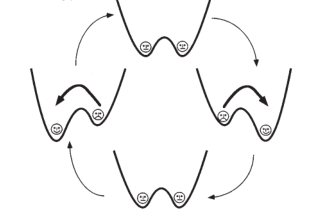
\includegraphics[width=20em]{000.png}
\caption{Incremental Domain Expansion: Illustration of the the
overall proposed learning framework. First a large margin embedding
(LME) detector is built based on labeled static images
from ImageNet. As unlabeled videos arrive, detected objects are
ranked based on detection confidence. Top ranked detections are
expanded into tracks and used for new class prototype learning.
Note that while a TV test sample (in red) may be too far in appearance
from the original ImageNet trained model and hence misclassified,
new prototypes, added based on tracks from videos, help to
bridge the gap leading to correct classification.
}
\label{fig:lable}
\end{figure}\\
\section{Related Work}
Domain extension method is closely related to domain adaptation. It is a statistical method, with emphasis on adapting existing models to a new domain in one domain. Domain adaptation can be classified as a supervised method, where tags can be applied to samples in the target domain and unsupervised methods, where tags are not provided\cite{Ferilli2013A}.\\

\section{Conclusion}
The problem of domain extension is solved, in which the range of the object detector that is learned on the training set of the initial image markup is extended incrementally to cover the incoming unlabeled video\cite{Li2007A}. An online probabilistic multi center large margin embedded model with detection constraints is a new model in which each object category is represented by multiple prototypes. With the self determined step learning algorithm selecting confidence samples from the confidence samples, the number is increasing\cite{Yi2008An}. The incoming unlabeled data is added.\\

{\small
\bibliographystyle{ieee}
\bibliography{1}
}
\end{document}
